\chapter{Results and Discussion}
\label{chapter:results}

In this chapter, I evaluate the performance of my architecture on the GQA dataset using a combination of traditional accuracy measures and GQA-specific metrics. First, I compare my architecture to the collection of baseline VQA methods introduced in the previous chapter. Secondly, I present results for variations of my model, replacing or entirely removing its question and/or scene graph processing modules to justify my architecture design. Finally, I delve into the parameter configuration of my model, exploring how parameters such as learning rate, reasoning module length and scene graph module size affect the performance of my model and the methods I used to find my final parameter configuration.

\section{Performance Evaluation}
\label{section:performance_evaluation}

\begin{table}[htbp]
    \begin{footnotesize}
        \begin{tabularx}{\linewidth}{L|c|cc|ccc}
            \toprule
            \multirow{2}{*}{\textbf{Model}} & \multicolumn{6}{c}{\textbf{GQA}} \\
            \cmidrule{2-7}
            & Accuracy & Binary & Open & Validity & Plausibility & Distribution \\
            \midrule
            Human \cite{hudson2019gqa} & 89.30 & 91.20 & 87.40 & 98.90 & 97.20 & - \\
            \midrule
            LXMERT \cite{tan2019lxmert, tan2019lxmertgithub}& 59.80 & - & - & - & - & - \\
            BAN-4 \cite{kim2018bilinear, guo2019bilinear} & 61.95 & - & - & - & - & - \\
            GRN \cite{guo2019bilinear} & 64.22 & - & - & - & - & - \\
            % MCAN \cite{yu2019deep, farazi2020attention} & 65.00 & 82.08 & 48.98 & 94.91 & 91.42 & 4.21\\
            MSA\cite{farazi2020attention} & 65.93 & 82.35 & 49.27 & 94.98 & 91.57 & 4.88\\
            \midrule
            MSA\(^{\dag}\) \cite{farazi2020attention} & 68.71 & 71.84 & 68.71 & 94.94 & 92.99 & 7.29\\
            MAC\(^\dag\) \cite{hudson2018compositional} & 73.64 & 81.86 & 65.94 & \textbf{95.38} & 92.46 & 2.05 \\
            MSA\(^{\ddag}\) \cite{farazi2020attention} & 81.15 & 85.06 & 77.48 & \textbf{95.34} & 94.26 & 1.08\\
            \midrule
            \textbf{Our Model}\(^\dag\) & \textbf{90.30} & \textbf{91.59} & \textbf{89.10} & \textbf{95.35} & \textbf{94.48} & \textbf{0.29} \\
            \bottomrule
        \end{tabularx}
        \caption[A performance comparison of various models on the GQA validation set.]{A comparison of the performance of various models on the GQA validation set. Human performance is based on majority vote of 5 human responses for 4000 random GQA questions. Models marked with a \(^\dag\) have access to pre-annotated GQA scene graph objects, attributes and relations at inference time, and models marked with a \(^\ddag\) use Faster R-CNN \cite{ren2016faster} features and/or bounding box information in addition to scene graph information. Where two citations are provided, the first corresponds to the original paper and the second corresponds to the source of the validation set results.}
        \label{table:performance_comparison}
    \end{footnotesize}
\end{table}

As demonstrated in \tableautorefname{ \ref{table:performance_comparison}}, my model outperforms all baseline models by a significant margin across all accuracy metrics, and performs on par or slightly better than reported models for GQA validity, plausibility and distribution. Moreover, it outperforms human baseline performance for all accuracy measures.

For fairness of comparison, I split baseline model performance into two sections; all models in the upper section use only Faster R-CNN and/or bounding box information during evaluation time, where all models in the lower section have access to GQA scene graph object, attribute and relationship data.

Stepping through each of the baselines in the upper section of \tableautorefname{ \ref{table:performance_comparison}}, it becomes evident how important the type of visual signal is for VQA models; we see that my model outperforms all four baselines that only have access to object and bounding box features by anywhere from 30.5\% in the case of LXMERT \cite{tang2019learning} to 24.37\% in the case of MSA \cite{farazi2020attention} when comparing overall accuracy. Since I use pre-annotated scene graphs from the GQA dataset as my model's visual signal, it makes sense that my model outperforms existing baselines that don't have access to this information. Moreover, we see that whilst my model outperforms MSA by 24.37\% in overall accuracy, the difference between the two models closes to only 9.24\% for binary-type questions, but grows to almost 50\% for open-type questions. Moreover, we see that my model has a much lower distribution than MSA, meaning it relies less on statistical priors in the dataset when forming its answers, and more on its visual input. Again, this is easily explained by the advantage of pre-annotated scene graph information. Interestingly, the difference in performance between my model and MSA on the validity and plausibility metrics is much less pronounced, at only 0.37\% and 2.91\% respectively. This is due to two primary reasons:

\begin{itemize}
    \item Validity and plausibility are much more forgiving metrics than accuracy. Validity is the most forgiving, since a model only has to provide an answer of the correct type \textit{e.g. provide a colour when the question about the colour of an object}. Plausibility is less forgiving than validity but still more forgiving than accuracy, since the provided answer has to make sense given the context of the question and image. As a result, the difference between validity for the two models is the smallest, followed by plausibility and then finally accuracy.
    \item Providing a valid or plausible answer does not always require visual information. We see this phenomenon in the results on the GQA test set in the original GQA publication \cite{hudson2019gqa}, where a language only LSTM model provides valid answers between 0.37\% and 0.21\% more often than the CNN + LSTM, BottomUp \cite{anderson2018bottom} and MAC \cite{hudson2018compositional} baselines, and provides plausible answers between 2.73\% and 3.05\% more often. Consequently, despite having a much weaker visual signal than my model, the MSA model in the upper section of \tableautorefname{ \ref{table:performance_comparison}} still performs comparably on the validity and plausibility metrics.
\end{itemize}

These observations extend to models in the lower section of \tableautorefname{ \ref{table:performance_comparison}}, which perform almost identically to my model on the validity metric, and between 0.2-2.0\% worse than my model for answer plausibility.

Moving our focus to the lower section of \tableautorefname{ \ref{table:performance_comparison}}, we see that the baseline models perform much better than those in the upper section, as they also have GQA scene graph information at their disposal. Importantly, we see that my model is still over 9.1\% more accurate than MSA despite not using any Faster R-CNN object features. When we remove Faster R-CNN features from MSA, we see a drop of almost 13\%, making my model almost 22.6\% more accurate than MSA given the same underlying information. Moreover, a MAC network that uses the same question encoding method as my model and uses GloVe embeddings for scene graph object, attributes and relations is still outperformed by my model by almost 16.7\%, highlighting the importance of the scene graph embedding and processing module in my final model.

Examining accuracy for binary and open question types, we see that while all three models that use scene graph information have a significantly lower (between 3.1-7.5\%) open-type accuracy compared to their binary-type accuracy, my model answers binary and open questions almost equally well, with only a 2.49\% difference between the two.

% TODO save for MSA
% Even though LXMERT \cite{tang2019learning} utilises the renowned transformer encoder \cite{vaswani2017attention} to embed visual Faster R-CNN and bounding box region features, it still has the arduous task of reconciling visual information with information from the question. Transformers have proven to be extremely capable in the Natural Language Processing (NLP) field, as their attention mechanisms operate well when their inputs are drawn from the same semantic space. Unfortunately, it is still not well-known how well scaled dot-product attention mechanisms like those found in transformers perform in multi-modal contexts, meaning the cross-modal transformer architecture used by LXMERT may have a hard time reconciling textual and visual features. Conversely, my model embeds both textual and visual information using GloVe vectors \cite{pennington2014glove}, meaning that both question and scene graph features are similar in their distributions and can consequently be compared easily using attention mechanisms. Consequently, my model performs an incredible 30.50\% better than LXMERT, however I posit that if LXMERT was to use similar embeddings for both textual and visual data, this gap would close significantly.

Based on the results in \tableautorefname{ \ref{table:performance_comparison}}, I believe the primary contributor to my model's excellent performance is its scene graph embedding and processing method. All three models in the lower half of the table use semantic word embeddings to represent scene graph objects, relations and attributes, and use attention-based reasoning methods. Consequently, the main point of differentiation between my model and the others is the use of graph attention networks (GATs) to process scene graph information. I confirm this hypothesis in \subsectionautorefname{ \ref{subsec:scene_graph_module_ablations}}, where I implement multiple scene graph processing module alternatives and demonstrate the effectiveness of GATs for learning semantically-rich scene graph embeddings.

\section{Ablation Studies}
\label{sec:ablation_studies}

To gain a more complete understanding of how the components of my model contribute to its performance, I explore how removing or replacing certain parts of my model change its behaviour. More specifically, I report how changes to the question processing module and scene graph processing module affect the performance of my model, investigating performance at a macro level using the metrics seen in the previous section, as well as at a micro level, examining model accuracy as a function of question length, question complexity and question structural and semantic types.  

For all ablation studies in this chapter, I train models on the balanced GQA training set and split the balanced GQA validation set in half, reserving the first half for parameter optimisation and the second half for testing. Consequently, all results reported in this section are computed on the second half of the balanced GQA validation set, instead of the full validation set like in \tableautorefname{ \ref{table:performance_comparison}}, to avoid giving an unfair advantage to my best model, which was tuned using the first half of the balanced validation set.

Before delving into ablation study results, it is important to understand the underlying distributions of the test set used to compute various metrics. As demonstrated in \tableautorefname{ \ref{tab:test_semantic_type_distribution}} and \tableautorefname{ \ref{tab:test_structural_type_distribution}}, the second half of the GQA validation set has a very similar semantic and structural type distribution to the rest of the balanced GQA dataset, as reported in \cite{hudson2019gqa_preprint}.

 Examining the distribution of semantic question types, we see that 46.6\% of questions query about the relationships between objects, 31.8\% ask about attributes, 11.8\% about objects, 6.6\% about object categories and 3.1\% about global properties. Regarding structural types, 51.7\% of questions are open-type questions that query about scene properties in general, 20.7\% of questions require verifying some property about the scene, 12.3\% require logical reasoning operations, 12.2\% require choosing between a set of options provided in the question and 3.1\% require comparing the properties of two or more objects.

% \begin{figure}[htbp]
%     \centering
%     \begin{subfigure}[l]{0.4\textwidth}
%         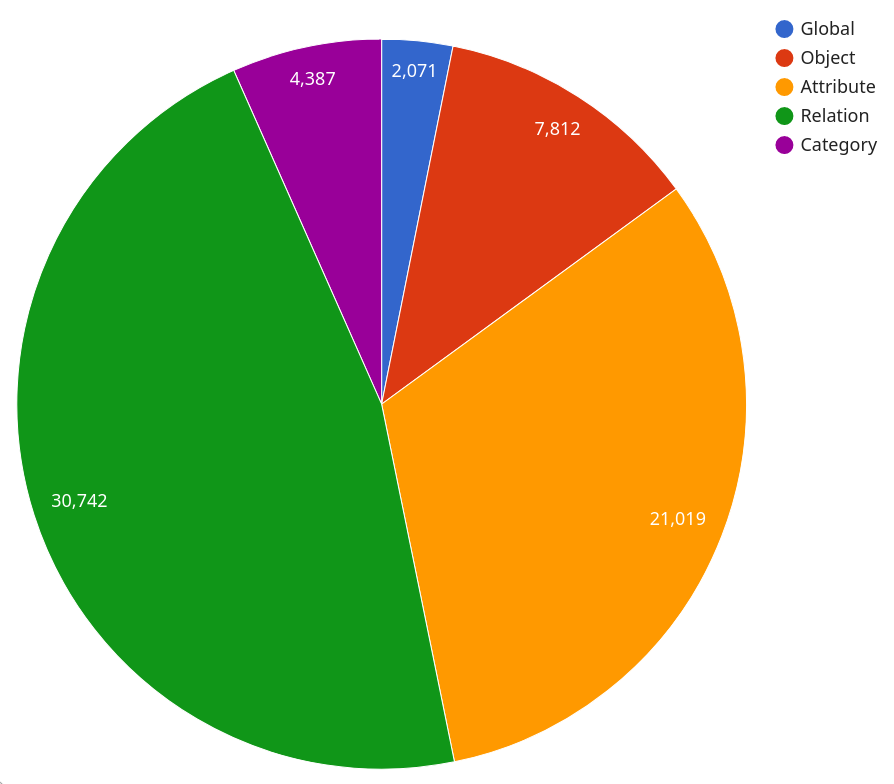
\includegraphics[width=\textwidth]{gqa_semantic_types.png}
%         \label{fig:test_semantic_types}
%         \caption{GQA semantic type distribution.}
%     \end{subfigure}
%     \begin{subfigure}[r]{0.4\textwidth}
%         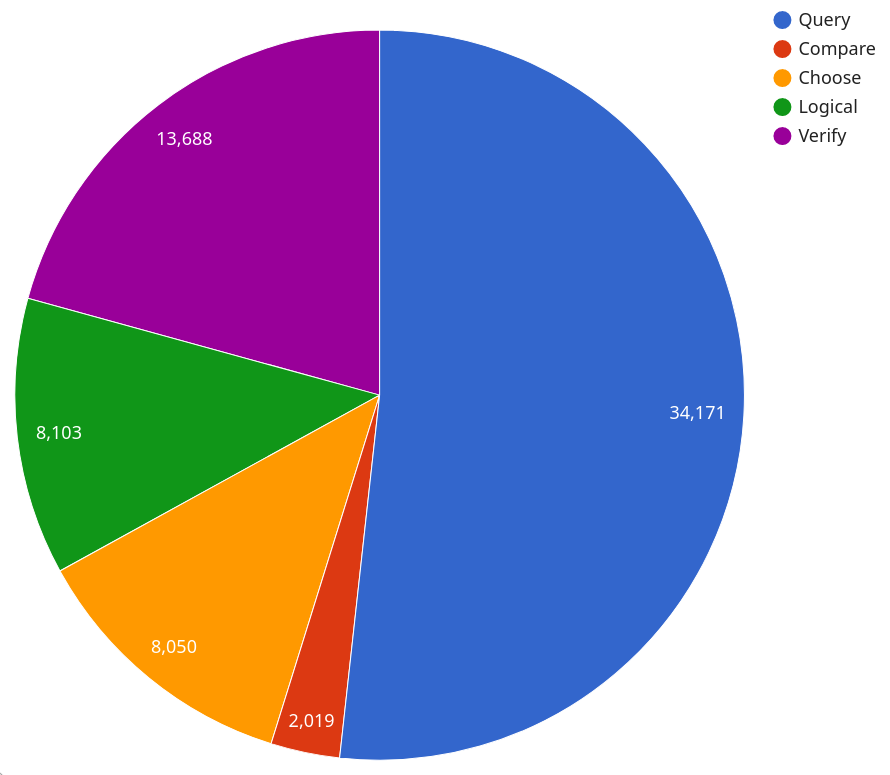
\includegraphics[width=\textwidth]{gqa_structural_types.png}
%         \label{fig:test_structural_types}
%         \caption{GQA structural type distribution.}
%     \end{subfigure}
%     \caption[GQA structural and semantic question type distributions.]{Distribution of structural and semantic question types across the second half of the balanced GQA validation set.}
%     \label{fig:test_structural_and_semantic_distribution}
% \end{figure}

\begin{table}[htbp]
    \centering
    \begin{tabular}{ccc}
        \toprule
        \textbf{Semantic Type} & \textbf{Count} & \textbf{Proportion}\\
        \midrule
        Relation & 30,742& 46.6\%\\
        Attribute & 21,019 & 31.8\%\\
        Object & 7,812 & 11.8\%\\
        Category & 4,387 & 6.6\%\\
        Global & 2,071 & 3.1\%\\
        \bottomrule
    \end{tabular}
    \caption[GQA semantic question type distribution.]{Distribution of semantic question types across the second half of the balanced GQA validation set.}
    \label{tab:test_semantic_type_distribution}
\end{table}

\begin{table}[htbp]
    \centering
    \begin{tabular}{ccc}
        \toprule
        \textbf{Structural Type} & \textbf{Count} & \textbf{Proportion}\\
        \midrule
        Query & 34,171 & 51.7\%\\
        Verify & 13,688 & 20.7\%\\
        Logical & 8,103 & 12.3\%\\
        Choose & 8,050 & 12.2\%\\
        Compare & 2,019 & 3.1\%\\
        \bottomrule
    \end{tabular}
    \caption[GQA structural question type distribution.]{Distribution of structural question types across the second half of the balanced GQA validation set.}
    \label{tab:test_structural_type_distribution}
\end{table}

\figureautorefname{ \ref{fig:test_reasoning_step_and_question_length_distribution}} illustrates the compositional nature of the questions in the GQA dataset, with the majority of questions requiring 2-3 discrete reasoning steps to arrive at an answer. We also see that most questions contain around 5 to 11 words, however there are still a large number of longer questions that a good VQA model needs to be able to interpret.

\begin{figure}[htbp]
    \centering
    \begin{subfigure}[l]{0.5\textwidth}
        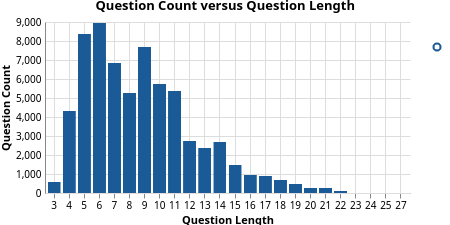
\includegraphics[width=\textwidth]{test_question_count_vs_question_length.png}
        \label{fig:test_question_length_distribution}
    \end{subfigure}
    \begin{subfigure}[r]{0.49\textwidth}
        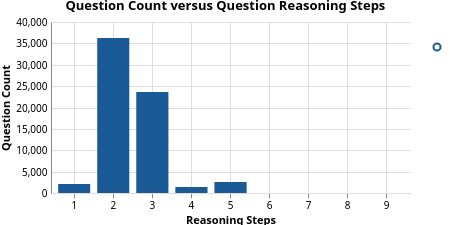
\includegraphics[width=\textwidth]{test_question_count_vs_reasoning_steps.png}
        \label{fig:test_reasoning_step_distribution}
    \end{subfigure}
    \caption[GQA question length and reasoning step count distributions.]{Distribution of questions across the second half of the balanced GQA validation set for both question length and reasoning step count.}
    \label{fig:test_reasoning_step_and_question_length_distribution}
\end{figure}



\subsection{Question Module Ablations}
\label{subsec:question_module_ablations}

In this \subsectionautorefname, I explore three alternative question processing modules, namely a convolutional neural network (CNN) inspired by work on sentence classification in the NLP field \cite{kim2014convolutional}, a graph convolutional network (GCN) that uses synactic dependencies as edges, and a graph attention network (GAT) that operates in a similar fashion to the GCN but learn individual weights for each syntactic dependency. Moreover, I investigate the effects of removing the question processing module entirely, relying purely on GloVe embeddings as a question input signal. Before delving into results, I provide a brief overview of how each of these ablations fit in to the rest of my model architecture, adopting notation from \chapterautorefname{ \ref{chapter:methodology}}.

\textbf{No question processing module}: For this ablation, I remove the scene graph module entirely, so the knpwledge-base of contextual question words \(K_{Q_{[i:i+k]}}\) is simply equal to the embedding feature matrix \(H_{Q_{[i:i+k]}}\). To obtain holistic question representations \(\mathcal{Q}_{Q_{[i:i+k]}}\), I simply average the embeddings of word features across the question length dimension of \(H_{Q_{[i:i+k]}}\).

\textbf{CNN}: Modeled on the architecture presented in \cite{kim2014convolutional}, the CNN question processing module takes a batch of raw question embeddings \(H_{Q_{[i:i+k]}} \in \R^{k \times l \times d_{H_q}}\) as its input and applies multiple 2D convolutions of varying receptive fields in parallel to learn a contextual representation of each question. I use a total of four Conv2D layers, each with 128 output channels and kernel sizes of \((3 \times d_{H_q})\), \((5 \times d_{H_q})\), \((7 \times d_{H_q})\) and \((9 \times d_{H_q})\). Appropriate padding is applied for each Conv2D layer so that convolved features for each layer are always of size \(l \times 128\). The convolved features for each layer are concatenated together to yield \(K_{Q_{[i:i+k]}} \in \R^{k \times l \times 512}\), the knowledge-base of contextual words used as an input to the reasoning module. After obtaining convolved features for each question in the batch, I take the maximum value of each output channel across the question length dimension to obtain a single vector \(\mathcal{Q}_q\) of dimension 512, representing the question as a whole. When processed as a batch, this yields a matrix of question representations \(\mathcal{Q}_{Q_{[i:i+k]} } \in \R^{k \times 512}\).

\textbf{GCN \& GAT}: As mentioned in \sectionautorefname{ \ref{section:question_embedding_and_module}}, I retrieve syntactic dependencies for each question using the Stanza NLP package \cite{qi2020stanza} during the question preprocessing stage. These syntactic dependencies form the edges of a question graph \(\mathcal{G}_q = (\mathcal{V}_q, \mathcal{E}_q)\), and the words of the question form the nodes. The type of syntactic dependency between individual words is ignored, as GCNs and GATs perform convolutions on nodes and not edges. Moreover, I ensure that \(\mathcal{G}_q\) is undirected, allowing messages to propagate through the dependency tree in both directions. To use this graph with GCN or GAT models, we need a node embedding matrix \(H_q \in \R^{l_q \times d_{H_q}}\) for each question \(q\) in the batch. These embeddings are obtained using the same question embedding technique described in \sectionautorefname{ \ref{section:question_embedding_and_module}}, but are batched differently. Instead of creating a dense batch of question embeddings \(H_{Q_{[i:i+k]}} \in \R^{k \times l \times d_{H_q}}\), I use the default PyTorch Geometric (PyG) \cite{fey2019fast} batching procedure, as described in \subsubsectionautorefname{ \ref{sec:scene_graph_embedding_details}}. Consequently, the output of the question embedding module is a batch of graphs \(\mathcal{G}_{Q_{[i:i+k]}}\) and associated batch of node embeddings, ready for input straight into a PyG GAT or GCN. Both the GAT and GCN question processing modules comprise 3 layers, with the first having an input size \(d_{H_q} = 300\) and the rest having input and output sizes of \(d_{K_q} = 256\). The GAT has the same head count and structure as the scene graph GAT module. For both the GAT and GCN, the final layer's output is converted to a dense batch of features and used as the question knowledge-base \(K_{Q_{[i:i+k]}} \in \R^{k \times l \times d_{K_q}}\). To obtain a batch of holistic question features, I use a global mean pooling operation on the final layer's output. These pooled features are converted to a dense batch of question embeddings \(\mathcal{Q}_{Q_{[i:i+k]}} \in \R^{k \times d_{K_q}}\). Both \(K_{Q_{[i:i+k]}}\) and\(\mathcal{Q}_{Q_{[i:i+k]}}\) are then passed to the reasoning module as usual.

\begin{table}[htbp]
\centering
\begin{footnotesize}
\begin{tabularx}{\linewidth}{CC|c|cc|ccc}
\toprule
\multirow{3}{0.1\textwidth}{\textbf{Question Module}} & \multirow{3}{0.1\textwidth}{\textbf{Scene Graph Module}} & \multicolumn{6}{c}{\multirow{2}{*}{\textbf{GQA}}}                                                                                                                                         \\
                                          &                                              & \multicolumn{6}{c}{}                                                                                                                                                                      \\ \cmidrule(l){3-8} 
                                          &                                              & \multicolumn{1}{l}{Accuracy} & \multicolumn{1}{l}{Binary} & \multicolumn{1}{l}{Open} & \multicolumn{1}{l}{Validity} & \multicolumn{1}{l}{Plausibility} & \multicolumn{1}{l}{Distribution} \\ \midrule
None                                      & GAT                                          & 86.52                        & 85.78                      & 87.21                    & 95.10                         & 93.85                            & 0.26                             \\
CNN                                       & GAT                                          & 87.35                        & 87.87                      & 86.86                    & 95.24                        & 94.22                            & 0.29                             \\
GCN                                       & GAT                                          & 86.02                        & 86.77                      & 85.32                    & 95.05                        & 93.92                            & 0.34                             \\
GAT                                       & GAT                                          & 89.43                        & \textbf{91.88}             & 87.16                    & 95.26                        & 94.19                            & 0.27                             \\
\midrule
BiLSTM                                    & GAT                                          & \textbf{90.45}               & 91.73                      & \textbf{89.26}           & \textbf{95.34}                        & \textbf{94.48}                   & \textbf{0.19}                    \\
\bottomrule
\end{tabularx}
\end{footnotesize}
\caption[Overall question processing module ablation performance.]{An overview of the impact of different question processing modules on overall model performance.}
\label{table:question_ablation_main}
\end{table}

As seen in \tableautorefname{ \ref{table:question_ablation_main}}, the BiLSTM question processing module outperforms all other question processing module types for total accuracy, open-type accuracy, validity, plausibility and distribution, and falls just shy (0.15\%) of the GAT question processing module on the binary accuracy metric. This is a testament to the expressive power of recurrent models for short sentences; the BiLSTM can capture relationships between all words in a given question regardless of its syntax, as it process each word in the question sequentially. In comparison, the effectiveness of the GAT and GCN question modules is highly dependent on the number of convolutional layers that they contain. Since each GAT or GCN layer can only propagate information to immediate neighbours of each node, the number of GAT or GCN layers must be equal or greater than the depth of the question's syntactic dependency tree to ensure that information can be shared between each word pair in the question. Whilst the CNN question module is capable of capturing contextual information about the question as a whole, it makes the assumption that related words occur near each other in the sentence, which is not always the case, especially for longer sentences. Since the CNN module was originally used for sentence classification \cite{kim2014convolutional}, I expect it learns useful holistic question representations \(\mathcal{Q}\), but struggles to capture relevant contextual information for individual words. This also explains why the CNN module performs slightly (0.83\%) better than the model variant with no question module at all, which simply takes the average of all embeddings for each word in the question as its holistic question representation \(\mathcal{Q}\).

In addition to the success of the BiLSTM question module, we also see that the relative ranking of the question modules is similar across all metrics, with BiLSTM performing the best, followed by the GAT module, then CNN, None and finally GCN. Whlst the GCN question module outperforms the model with no question processing module on the binary accuracy metric, it struggles to answer open-type questions. This is likely because it always propagates features between syntactically-connected question words, regardless of whether these syntactical relationships are important to the question or not. As a result, the expressive power of the GloVe embeddings initially used to embed each word is lost due to unwanted propagations between question words. On the other hand, the GAT question processing module outperforms both the GCN module and the bare GloVe embedding variation across all metrics, due to its ability to learn attention weights between question words. This helps it to learn better contextual word-level embeddings, which are essential for obtaining useful control vectors in the reasoning module.

\begin{table}[htbp]
\centering
\begin{footnotesize}
\begin{tabular}{cc|c|ccccc}
\toprule
\multirow{3}{0.1\textwidth}{\textbf{Question Module}} & \multirow{3}{0.1\textwidth}{\textbf{Scene Graph Module}} & \multicolumn{6}{c}{\multirow{2}{*}{\textbf{GQA}}}                                                   \\
                                          &                                              & \multicolumn{6}{c}{}                                                                                \\ \cmidrule(l){3-8} 
                                          &                                              & Accuracy       & Query          & Compare        & Choose         & Logical        & Verify         \\ \midrule
None                                      & GAT                                          & 86.52          & 87.21          & 80.44          & 78.89          & 93.77          & 85.88          \\
CNN                                       & GAT                                          & 87.35          & 86.86          & 67.66          & 85.99          & 92.57          & 89.17          \\
GCN                                       & GAT                                          & 86.02          & 85.32          & 73.60          & 84.96          & 92.85          & 86.17          \\
GAT                                       & GAT                                          & 89.43          & 87.16          & \textbf{93.02} & 86.92          & 96.43          & 91.93          \\
\midrule
BiLSTM                                    & GAT                                          & \textbf{90.45} & \textbf{89.26} & 69.69          & \textbf{90.87} & \textbf{97.45} & \textbf{92.10} \\ \bottomrule
\end{tabular}
\end{footnotesize}
\caption[Question processing module ablation performance for questions of differing structural types.]{An overview of the impact of different question processing modules on model accuracy for questions of differing structural types.}
\label{table:question_ablation_structural}
\end{table}

Moving our focus to \tableautorefname{ \ref{table:question_ablation_structural}}, we see that the performance of each question module variation on query-type questions coincides with their open-type question accuracy. Moreover, the performance of each question module on verify-type questions is within 1.5\% of their total binary-type question accuracy. Consequently, the BiLSTM question module outperforms other question processing module types for most structural types, with the exception of \textit{compare} type questions, where the GAT question module outperforms other question types by anywhere from 12.58\% to 25.36\%. Whilst it may be tempting to attribute the large decrease in performance for most question modules on compare-type questions to the fact that it is the least common structural question type at only 3.1\% of samples, we cannot ignore that the GAT question module performs so well. Referring back to \tableautorefname{ \ref{table:gqa_question_samples}} in the previous chapter, we see that comparison questions can be either binary or open, and most often ask about common or different properties of two objects. After inspecting the control unit attention weights for the GAT question module and the BiLSTM question module, we see that the GAT question module attends to entire phrases of the question like \textit{have the same colour}, where the BiLSTM question module attends to words like \textit{do} or \textit{is}, indicating it is relying on question priors information to formulate its answers. I provide an example of this in \appendixautorefname{ \ref{appendix:ablation_study_visualisations}}, \sectionautorefname{ \ref{section:question_processing_module_ablation_visualisations}}, showing the regions of the question and scene graph that the model attends to.

\begin{table}[htbp]
\centering
\begin{footnotesize}
\begin{tabular}{cc|c|ccccc}
\toprule
\multirow{3}{0.1\textwidth}{\textbf{Question Module}} & \multirow{3}{0.1\textwidth}{\textbf{Scene Graph Module}} & \multicolumn{6}{c}{\multirow{2}{*}{\textbf{GQA}}}                                                   \\
                                          &                                              & \multicolumn{6}{c}{}                                                                                \\ \cmidrule(l){3-8} 
                                          &                                              & Accuracy       & Global         & Object         & Attribute      & Relation       & Category       \\ \midrule
None                                      & GAT                                          & 86.52          & \textbf{83.97}          & 94.75          & 87.35          & 83.67          & 89.01          \\
CNN                                       & GAT                                          & 87.35          & 83.78          & 93.63          & 85.37          & 87.37          & 87.14          \\
GCN                                       & GAT                                          & 86.02          & 83.39          & 93.36          & 83.65          & 86.32          & 83.43          \\
GAT                                       & GAT                                          & 89.43          & 83.82          & 97.24          & \textbf{89.74} & 87.88          & 87.62          \\
\midrule
BiLSTM                                    & GAT                                          & \textbf{90.45} & 83.92          & \textbf{97.39} & 88.39          & \textbf{90.51} & \textbf{90.65} \\ \bottomrule
\end{tabular}
\end{footnotesize}
\caption[Question processing module ablation performance for questions of differing semantic types.]{An overview of the impact of different question processing modules on model accuracy for questions of differing semantic types.}
\label{table:question_ablation_semantic}
\end{table}

Examining \tableautorefname{ \ref{table:question_ablation_semantic}}, we see that all question modules perform comparably for questions with global targets. This is primarily due to the fact that there is no global scene information included in the visual signal, so it is difficult to answer questions about global scene properties regardless of the quality of the question representation. This also explains why the global accuracy is much lower than the overall accuracy for all question module types.

For questions that query about objects and/or attributes, we see that the GAT and BiLSTM question modules perform the best, as they are able to learn good contextual representations of individual question words, unlike CNN or GCN which are better at embedding the question representation as a whole. Additionally, we see a difference of around \(2.6\%\) between object-type accuracy of the BiLSTM question module and the model with no question module at all, indicating that some object-type questions require contextual question information, for example, they query about a \textit{red apple} as opposed to just an \textit{apple}.

For relationship-based questions, we observe again that the BiLSTM performs the best, outperforming the GAT and CNN and GCN question modules by 2.63\%, 3.14\% and 4.19\% respectively. This is primarily due to its ability to capture sequences of words where other question modules can't. This is essential for relations in the GQA dataset, as the two most common relationships are \textit{to the left of} and \textit{to the right of}, which the question module needs to be able to capture as single concepts. Furthermore, when we don't use any question module at all, we suffer a 6.84\% performance drop when compared to the BiLSTM question module, since the raw GloVe embeddings don't contain any contextual information.

Finally, for category-based questions, we see that GCN, CNN and GAT question modules all perform worse than not using a question module at all by anywhere from 1.39\% in the case of GAT through to 5.58\% in the case of the GCN question module. In general, category-type questions require associating a category with an object, \textit{e.g.} \textit{fruit} with \textit{banana}. As a result, it is essential that the category is represented adequately and not clouded by other parts of the question so the model can learn to search for related concepts in the scene graph.

\begin{figure}[htbp]
    \centering
    \begin{subfigure}[l]{0.5\textwidth}
        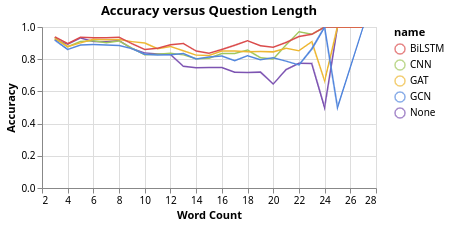
\includegraphics[width=\textwidth]{accuracy_vs_question_length_question_ablation.png}
        \label{fig:accuracy_vs_question_length_question_ablation}
    \end{subfigure}
    \begin{subfigure}[r]{0.49\textwidth}
        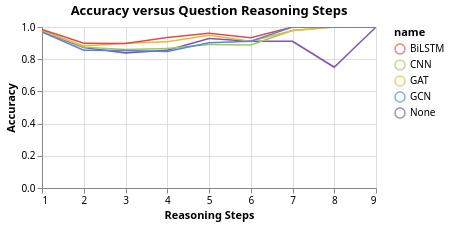
\includegraphics[width=\textwidth]{accuracy_vs_reasoning_steps_question_ablation.png}
        \label{fig:accuracy_vs_reasoning_steps_question_ablation}
    \end{subfigure}
    \caption{Per-question-length and per-reasoning-step accuracy for various question processing module types. The high performance of the right-hand tails in both cases are due to the small number of questions with a large number of words or reasoning steps, as illustrated in \figureautorefname{ \ref{fig:test_reasoning_step_and_question_length_distribution}}.}
    \label{fig:accuracy_vs_question_length_and_reasoning_steps_question_ablation}
\end{figure}

In \figureautorefname{ \ref{fig:accuracy_vs_question_length_and_reasoning_steps_question_ablation}}, we see that both GAT and BiLSTM question modules perform similarly as the number of reasoning steps required by the question increases, clearly outperforming alternative question modules. In addition, we see that as question length increases, question modules that use mean or max pooling to obtain a holistic representation tend to decrease in performance faster than the BiLSTM question module, which uses its concatenated forward and backward hidden layers as a question representation. When using no question module at all, performance decreases drastically as question length increases, since the mean of the question words use to represent the question becomes a less reliable embedding of the question as a whole.

\subsection{Scene Graph Module Ablations}
\label{subsec:scene_graph_module_ablations}

In this subsection, I investigate two alternative scene graph processing modules, namely a BiLSTM and a graph convolutional network (GCN). In addition, I inspect how removing the scene graph processing module affects overall performance, comparing results for these different architectures across a variety of metrics. Again, I provide a brief overview of how each of these ablations interact with rest of my model architecture, adopting relevant notation from \chapterautorefname{ \ref{chapter:methodology}}.

% In addition, I justify my choice to omit the non-linear activation function \(f\) from my GAT scene graph processing module (refer to \equationautorefname{ \ref{equation:gat_propagation_rule}}), comparing performance both with and without a LeakyReLU activation function. 

\textbf{No scene graph processing module}: For this ablation, I remove the scene graph processing module entirely. After constructing a scene graph \(\mathcal{G}_{R_{[i:i+k]}}\) and associated node feature matrix \(H_{R_{[i:i+k]}}\) in the scene graph embedding module, the node feature tensor is passed directly to the reasoning module. That is, I use the node feature tensor \(H_{R_{[i:i+k]}}\) as the knowledge-base of scene graph objects, attributes and relations \(K_{R_{[i:i+k]}}\), completely disregarding any edge information on \(\mathcal{G}_{R_{[i:i+k]}}\). Investigating the effect of edge information removal is essential for understanding how much of my model performance stems from the embedding of scene graph object, attribute and relation features versus how much is due to the contextual graph information learned by GAT layers.

\textbf{BiLSTM}: The BiLSTM scene graph processing module aims to capture contextual relationships between scene graph object, attribute and relation triples, without any structured graph-based information. Instead of building a matrix of node embeddings containing scene graph objects, attributes and relations, like in the regular scene graph embedding module, I create an input feature matrix \(H_r \in \R^{m \times d_{H_r}}\) for each scene graph \(r\) as follows: For each of the \(m_r\) objects in the scene graph \(r\), the \(i\)th row of \(H_r\) is the concatenation of three vectors \(u_i, v_i\) and \(w_i\), where \(u_i\) the \(i\)th object's GloVe embedding, \(v_i\) is the mean of the GloVe embeddings of the \(i\)th object's incoming and outgoing relations, and \(w_i\) is the mean of the GloVe embeddings of all attributes associated with object \(i\). In the event that an object contains no incoming or outgoing relations, or no attributes, I set \(v_i\) or \(w_i\) to a 300-dimensional zero vector respectively. All feature matrices are stached to form a single tensor \(H_{R_{[i:i+k]}} = [H_{r_i}, ..., H_{r_{i+k-1}}]\), which is in turn fed to a single-layer BiLSTM. Since each direction of the BiLSTM has a hidden size of 256, the concatenated last layer outputs of each direction form 512-dimensional vector for each of the \(m_r\) \(d_{H_r} = 900\) dimensional input vectors, denoted \(K_r\). These matrices are stacked to yield a knowledge-base of scene graph features for all graphs in the batch, denoted \(K_{R_{[i:i+k]}} \in \R^{k \times m \times d_{K_r}}\), where \(d_{K_r} = 512\) and \(m\) is the maximum number in any single scene graph in the batch. \(K_{R_{[i:i+k]}} \in \R^{k \times m \times d_{K_r}}\) is then passed to the reasoning module as usual.

\textbf{GCN}: The GCN scene graph processing module is identical in terms of inputs and outputs as the GAT scene graph processing module, except it uses GCN convolution operations instead of GAT convolutions. Since GCNs have no attention heads, each GCN layer operates on all features of the input instead of a quarter of the input each in the case of GAT with four attention heads.

\begin{table}[htbp]
\centering
\begin{footnotesize}
\begin{tabularx}{\linewidth}{CC|c|cc|ccc}
\toprule
\multirow{3}{0.1\textwidth}{\textbf{Question Module}} & \multirow{3}{0.1\textwidth}{\textbf{Scene Graph Module}} & \multicolumn{6}{c}{\multirow{2}{*}{\textbf{GQA}}}                                                                                                                                         \\
                                          &                                              & \multicolumn{6}{c}{}                                                                                                                                                                      \\ \cmidrule(l){3-8} 
                                          &                                              & \multicolumn{1}{l}{Accuracy} & \multicolumn{1}{l}{Binary} & \multicolumn{1}{l}{Open} & \multicolumn{1}{l}{Validity} & \multicolumn{1}{l}{Plausibility} & \multicolumn{1}{l}{Distribution} \\ \midrule
BiLSTM                                    & None                                         & 73.63                        & 81.84                      & 65.98                    & \textbf{95.38}               & 92.46                            & 1.09                    \\
BiLSTM                                    & BiLSTM                                       & 83.35                        & 85.81                      & 81.06                    & 95.27                        & 93.73                            & 0.31                             \\
BiLSTM                                    & GCN                                          & 69.44                        & 78.14                      & 61.34                    & 95.13                        & 91.95                            & 1.11                             \\
\midrule
BiLSTM                                    & GAT                                          & \textbf{90.45}               & \textbf{91.73}                      & \textbf{89.26}           & \textbf{95.34}                        & \textbf{94.48}                   & \textbf{0.19}                    \\
\bottomrule
\end{tabularx}
\end{footnotesize}
\caption[Overall scene graph processing module ablation performance.]{An overview of the impact of different scene graph processing modules on overall model performance.}
\label{table:scene_graph_ablation_main}
\end{table}

The importance of an effective scene graph processing module is clearly outlined in \tableautorefname{ \ref{table:scene_graph_ablation_main}}, where we see just how successful the GAT architecture is at capturing contextual scene graph information. The GAT scene graph processing module outperforms all other processing modules on all three accuracy measures, as well as for plausibility and distribution. We see similar comparable results for validity regardless of the scene graph module type, for the same reasons introduced in \sectionautorefname{ \ref{section:performance_evaluation}}.

We see improvements almost 17\% on overall accuracy, almost 10\% on binary-type accuracy and over 23\% on open-type by processing scene graph features with a GAT prior to the reasoning module, and increase the plausibility of answers by just over 2\%. Without the GAT to process scene graph edges, the reasoning module simply receives a list of all objects, attributes and relations in the scene and is not provided with any context about which attributes and relationships are associated with which objects. Consequently, these large performance gains are solely due to GAT's ability to implicitly capture scene graph edge information and embed the interactions between object, attribute and relation nodes prior to performing reasoning operations.

The BiLSTM scene graph processing module achieves the second-highest performance across all metrics, falling just over 7\% shy of the GAT processing module on the overall accuracy metric, but ourperforming both the GCN scene graph module and no scene graph module model variants. This is primarily a result of explicitly concatenating an object's relation and attribute information with the embedding of the object itself, as this allows the reasoning module to answer questions about the attributes and relationships of a particular object. Naturally, this method of expressing object, attribute and relationship data is far from optimal, but it performs surprisingly well despite its naivety.

Finally, we see that the GCN scene graph processing module performs extremely poorly. Not using a scene graph processing module at all results in an almost 4.2\% overall increase in accuracy and a 0.5\% increase in answer plausibility. These results show that even though the GCN knows which node embeddings are related, it is ineffective at capturing those relationships as node features due to its inability to attend to some relationships more than others.

\begin{table}[htbp]
\centering
\begin{footnotesize}
\begin{tabular}{cc|c|ccccc}
\toprule
\multirow{3}{0.1\textwidth}{\textbf{Question Module}} & \multirow{3}{0.1\textwidth}{\textbf{Scene Graph Module}} & \multicolumn{6}{c}{\multirow{2}{*}{\textbf{GQA}}}                                                   \\
                                          &                                              & \multicolumn{6}{c}{}                                                                                \\ \cmidrule(l){3-8} 
                                          &                                              & Accuracy       & Query          & Compare        & Choose         & Logical        & Verify         \\ \midrule
BiLSTM                                    & None                                         & 73.63          & 65.98          & 69.44          & 72.84          & 92.85          & 82.44          \\
BiLSTM                                    & BiLSTM                                       & 83.35          & 81.06          & \textbf{92.22}          & 73.98          & 95.79          & 85.91          \\
BiLSTM                                    & GCN                                          & 69.44          & 61.34          & 66.37          & 71.04          & 85.96          & 79.43          \\
\midrule
BiLSTM                                    & GAT                                          & \textbf{90.45} & \textbf{89.26} & 69.69          & \textbf{90.87} & \textbf{97.45} & \textbf{92.10} \\ \bottomrule
\end{tabular}
\end{footnotesize}
\caption[Scene graph processing module ablation performance for questions of differing structural types.]{An overview of the impact of different scene graph processing modules on model accuracy for questions of differing structural types.}
\label{table:scene_graph_ablation_structural}
\end{table}

Progressing to \tableautorefname{ \ref{table:scene_graph_ablation_structural}}, we see that the relative rankings of each of the scene graph modules for query, choose, logical and verify question types are the same as for overall accuracy, with GAT outperforming BiLSTM, and GCN performing worse than raw GloVe embeddings. We see that the query-type accuracy for all four modules is identical to the open-type accuracy presented in \tableautorefname{ \ref{table:scene_graph_ablation_main}}, and the verify-type accuracy is similar to the binary-type accuracy. We see a 5.6\% performance increase on choose-type questions when using a GAT to process node features instead of using the features directly, but more interestingly, we see a minimal increase in performance by using the BiLSTM scene graph processing module over raw node features despite the BiLSTM module having access to the concatenated object, attribute and relation features that caused a 9.7\% increase on overall accuracy. This likely occurs because the concatenated features only capture first-order interactions between scene graph objects, relations and attributes; given the relationship \textit{(man, to the left of, dog)}, the BiLSTM scene graph processing module knows that the man is to the left of something, and the dog has something to the left of it, but there is no way of knowing that the man is related to the dog. Since most choose-type questions require choosing between two objects based on attributes or relationships, we see that the BiLSTM module only sees a slight 1.1\% performance gain over not using a scene graph processing module at all.

For compare-type questions, the GAT and GCN scene graph modules perform poorly at 69.69\% and 66.37\% respectively, where the BiLSTM scene graph module performs outstandingly well. Since the BiLSTM module uses concatenated object, attribute and relation features, compare-type questions about attributes like \textit{Are the shirt and the flower the same colour?} are much easier to answer, since the reasoning module only has to identify the relevant objects by their embeddings and then compare the attribute portion of the concatenated vector. For other scene graph processing types, the reasoning module has to first locate the objects, and then use precious reasoning steps to query their colours before comparing them to retrieve an answer.

\begin{table}[htbp]
\centering
\begin{footnotesize}
\begin{tabular}{cc|c|ccccc}
\toprule
\multirow{3}{0.1\textwidth}{\textbf{Question Module}} & \multirow{3}{0.1\textwidth}{\textbf{Scene Graph Module}} & \multicolumn{6}{c}{\multirow{2}{*}{\textbf{GQA}}}                                                   \\
                                          &                                              & \multicolumn{6}{c}{}                                                                                \\ \cmidrule(l){3-8} 
                                          &                                              & Accuracy       & Global         & Object         & Attribute      & Relation       & Category       \\ \midrule
BiLSTM                                    & None                                         & 73.63          & \textbf{85.18} & 95.15          & 64.46          & 72.38          & 82.54          \\
BiLSTM                                    & BiLSTM                                       & 83.35          & 82.86          & 95.60          & 80.88          & 81.02          & 89.92          \\
BiLSTM                                    & GCN                                          & 69.44          & 70.45          & 87.54          & 67.22          & 66.25          & 69.77          \\
\midrule
BiLSTM                                    & GAT                                          & \textbf{90.45} & 83.92          & \textbf{97.39} & \textbf{88.39}          & \textbf{90.51} & \textbf{90.65} \\
\bottomrule
\end{tabular}
\end{footnotesize}
\caption[Scene graph processing module ablation performance for questions of differing semantic types.]{An overview of the impact of different scene graph processing modules on model accuracy for questions of differing semantic types.}
\label{table:scene_graph_ablation_semantic}
\end{table}

In \tableautorefname{ \ref{table:scene_graph_ablation_semantic}}, we see that the GAT scene graph processing module outperforms alternative scene graph processing methods for all question semantic types except questions about global scene information. Interestingly, when using no scene graph processing module, we observe a 1.26\% increase in global question-type accuracy over the GAT scene graph module. This indicates that raw GloVe embeddings provide a useful signal for establishing global scene properties such as weather and location; for example, a scene that contains embeddings for \textit{sky}, \textit{cloud} and \textit{umbrella} objects is likely outdoors.

For questions about objects, we see that the GAT scene graph module outperforms the GCN module by almost 10\% indicating the importance of attention weights in establishing which object, attribute and relationship interactions are important. Moreover, the GAT module outperforms the BiLSTM module and raw GloVe features by almost 1.7\% and 2.2\% respectively, indicating the benefits of enriching object features with attribute and relationship information. We see that the GCN module performs poorly again, at 21.17\% and 24.26\% worse than the GAT module for questions about attributes and relations respectively. As expected, the absence of a scene graph processing module makes it difficult to associate relation or attribute features with an object, explaining the poor attribute-type and relation-type accuracies when using only GloVe embeddings. As discussed previously, the BiLSTM scene graph module is able to capture first order interactions between objects and their attributes and/or relations, but struggles to capture second-order interactions, explaining the 7.51\% and 9.49\% performance decrease for questions about attributes and relations when compared to the GAT module.

\begin{figure}[htbp]
    \centering
    \begin{subfigure}[l]{0.5\textwidth}
        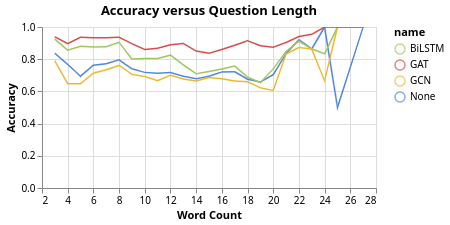
\includegraphics[width=\textwidth]{accuracy_vs_question_length_scene_graph_ablation.png}
        \label{fig:accuracy_vs_question_length_scene_graph_ablation}
    \end{subfigure}
    \begin{subfigure}[r]{0.49\textwidth}
        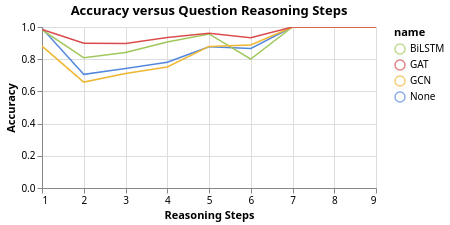
\includegraphics[width=\textwidth]{accuracy_vs_reasoning_steps_scene_graph_ablation.png}
        \label{fig:accuracy_vs_reasoning_steps_scene_graph_ablation}
    \end{subfigure}
    \caption{Per-question-length and per-reasoning-step accuracy for various scene graph processing module types. The high performance of the right-hand tails in both cases are due to the small number of questions with a large number of words or reasoning steps, as illustrated in \figureautorefname{ \ref{fig:test_reasoning_step_and_question_length_distribution}}.}
\end{figure}

\figureautorefname{ \ref{fig:accuracy_vs_reasoning_steps_scene_graph_ablation}} demonstrates the response of different scene graph processing modules to question length and complexity. As expected, the GAT module outperforms the other modules, and maintains reasonable performance as question length and reasoning step count increases. Moreover, we see that the GCN consistently decreases the performance of the model as a whole, regardless of question length or complexity. The BiLSTM module performs well for smaller question lengths and smaller reasoning step counts, but its performance rapidly decreases as the question word count increases. This is primarily due to its inability to capture interactions between objects as previously discussed, as these interactions are more common in longer questions.

\section{Hyperparameter Optimisation}
\label{sec:hyperparameter_optimisation}

Rigorous initial tests were performed - reported and non-reported results represent 159 days of GPU computation time.

These results represent a total of 55 days of GPU compute

{\color{red}
  \begin{itemize}
    \item \textit{Weights \& Biases} \cite{wandb} implementation of bayesian optimisation, using the hyperband early stopping method
    \item Include results using LeakyReLU between GAT layers?
  \end{itemize}
}



The effects of the Hyperband method are clearly seen in \figureautorefname{ \ref{fig:hyperparameter_optimisation_validation_loss_and_accuracy}}, where only a few models are trained to completion and less promising models are stopped earlier to encourage exploration of the hyperparameter search space.

\begin{figure}
    \centering
    \begin{subfigure}[t]{\textwidth}
        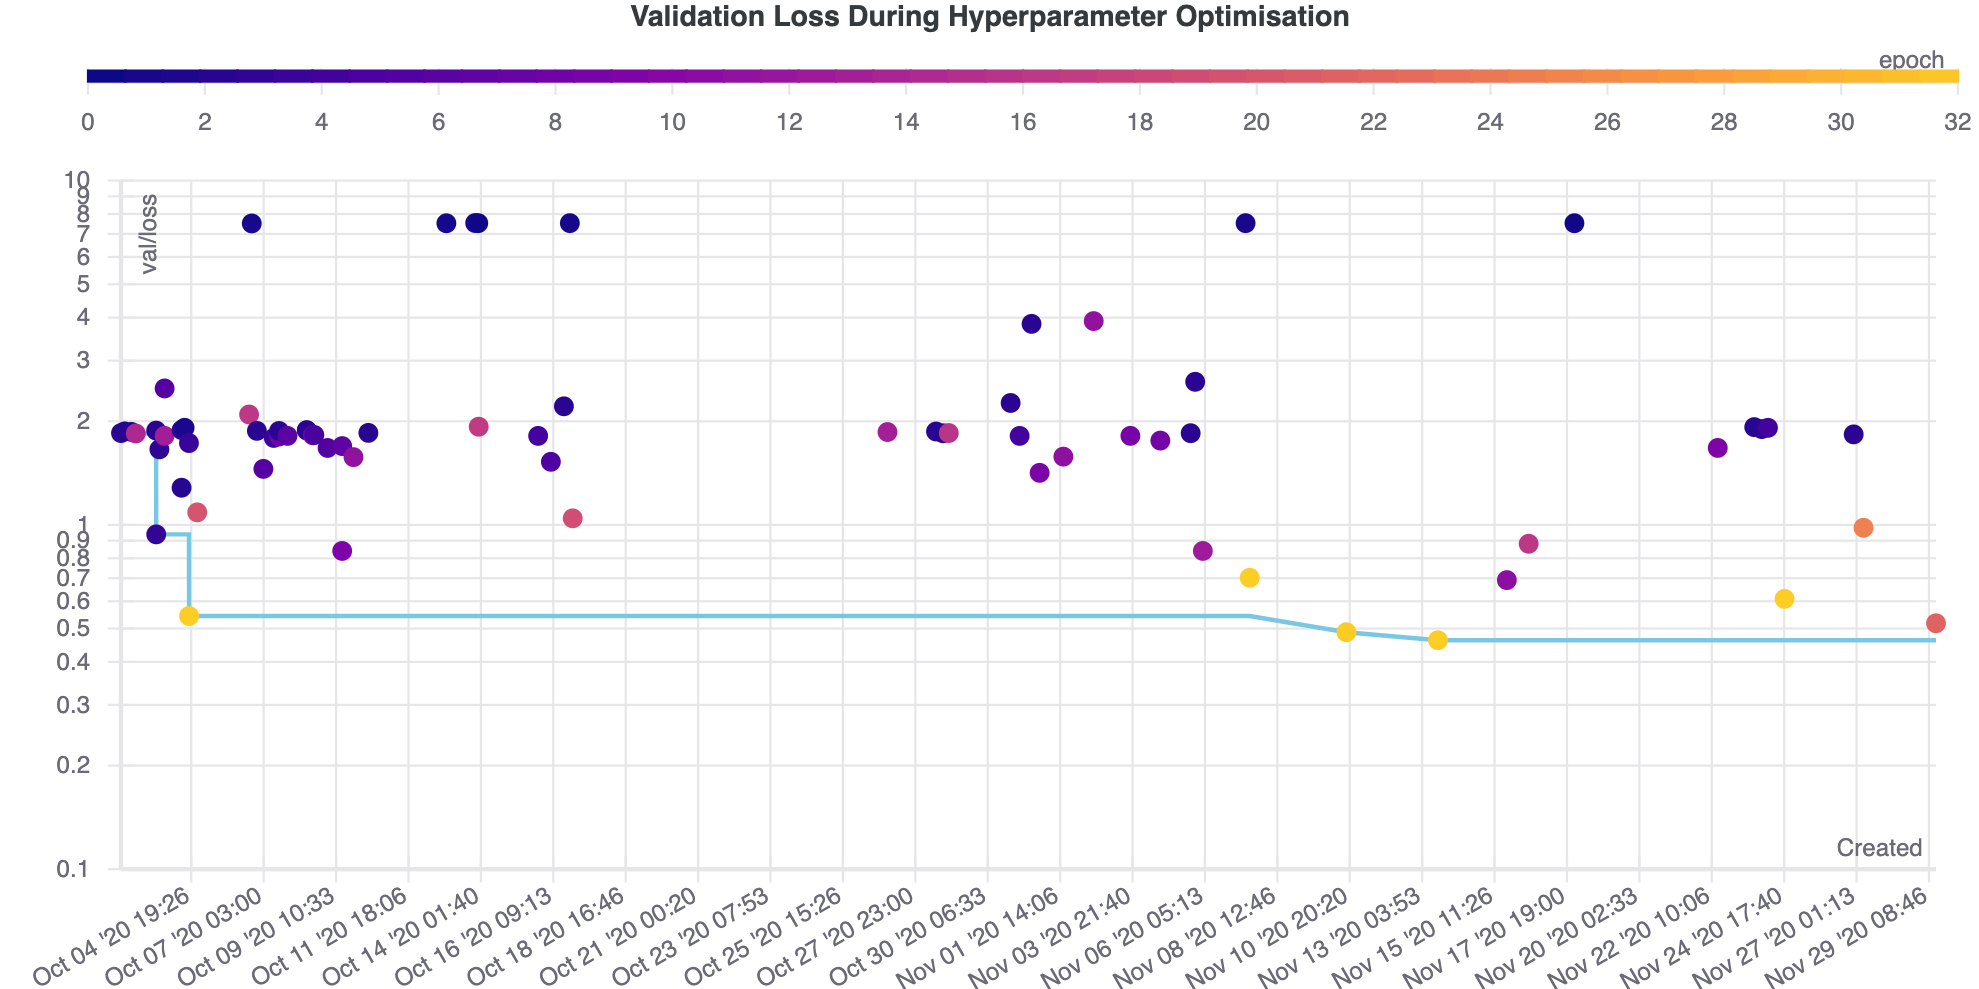
\includegraphics[width=\textwidth]{hyperparameter_optimisation_validation_loss.png}
        \label{fig:hyperparameter_optimisation_validation_loss}
        \caption{Validation loss throughout the hyperparameter optimisation process.}
    \end{subfigure}
    \par\bigskip % force a bit of vertical whitespace
    \par\bigskip
    \begin{subfigure}[b]{\textwidth}
        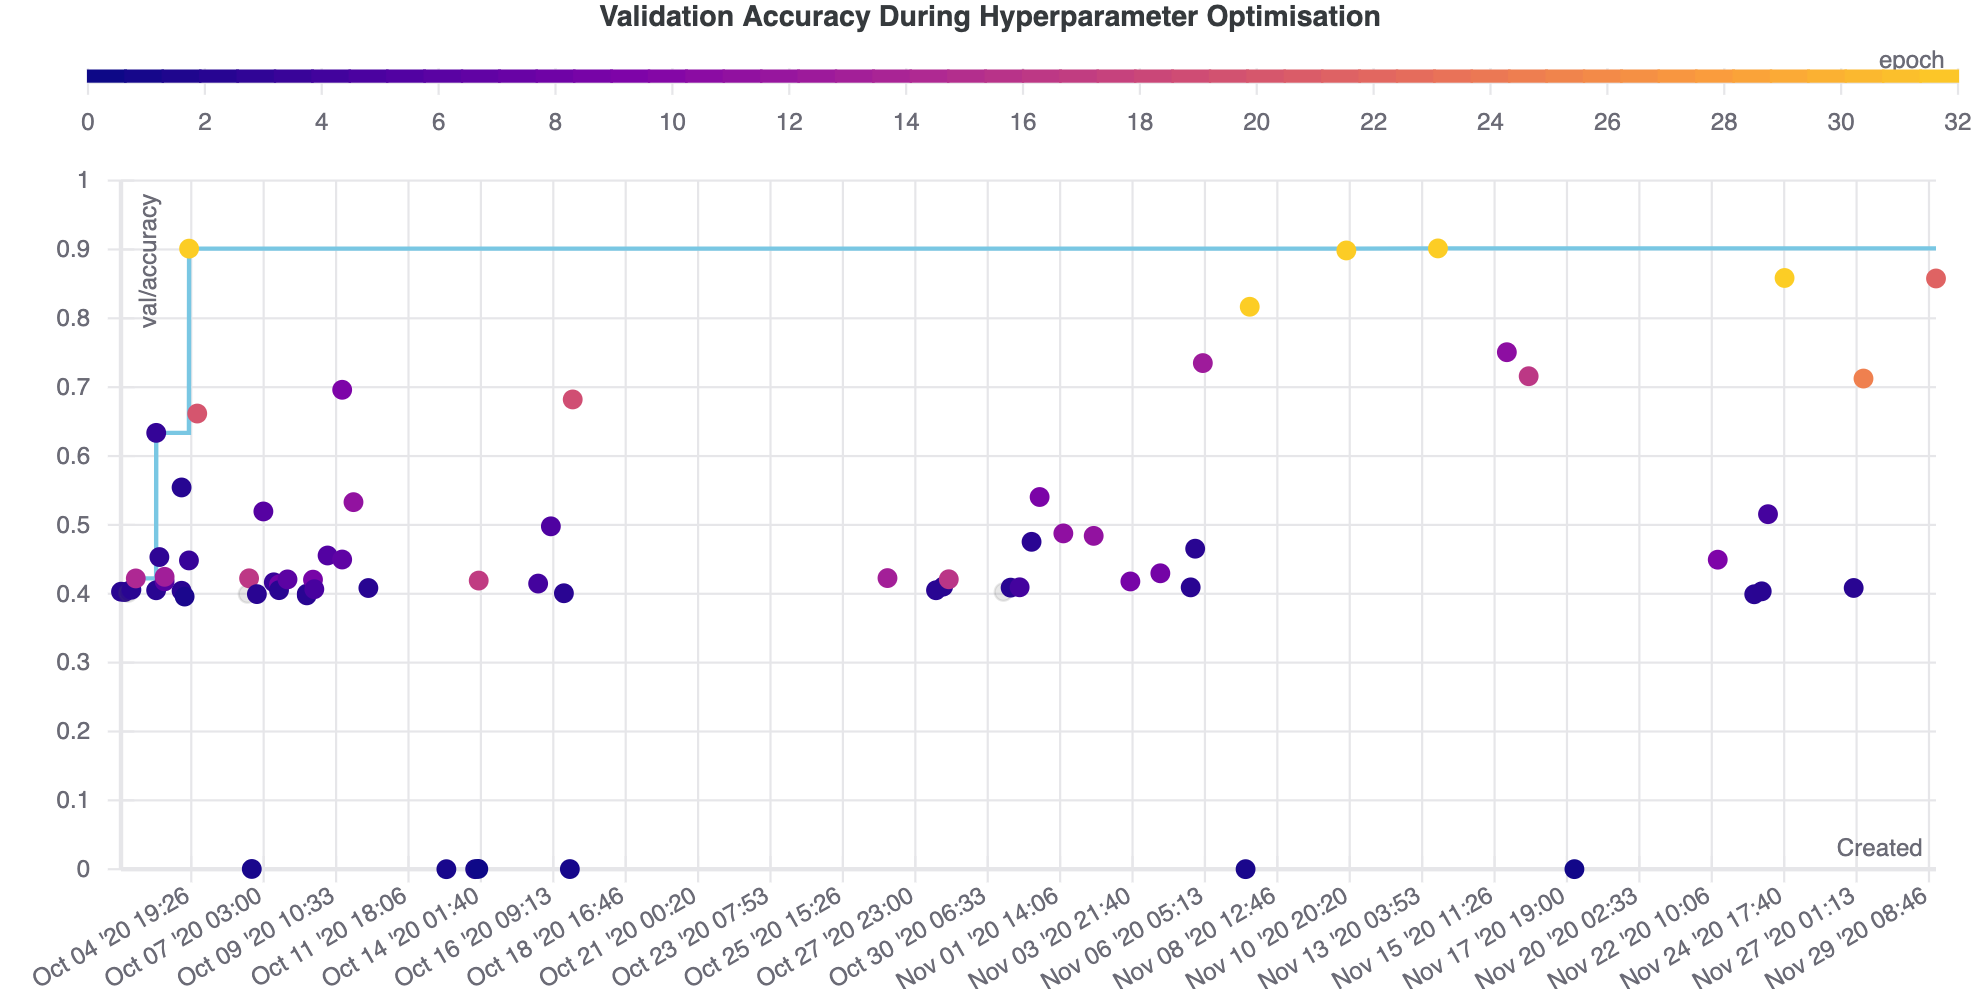
\includegraphics[width=\textwidth]{hyperparameter_optimisation_validation_accuracy.png}
        \label{fig:hyperparameter_optimisation_validation_accuracy}
        \caption{Validation accuracy throughout the hyperparameter optimisation process. Greyed out points correspond to models with a loss greater than 10.}
    \end{subfigure}
    \caption{A summary of validation loss and accuracy throughout the hyperparameter optimisation process. Each point represents a trained model, and its colour indicates how many epochs the model was trained for.}
    \label{fig:hyperparameter_optimisation_validation_loss_and_accuracy}
\end{figure}

\begin{figure}
    \centering
    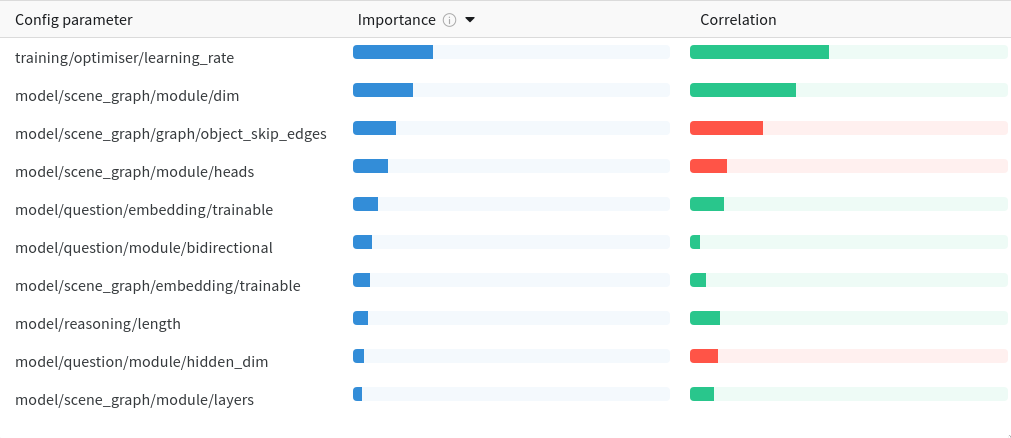
\includegraphics[width=\textwidth]{hyperparam_importance_and_correlation.png}
    \caption{Hyperparameter importance with respect to validation loss. Correlation is the linear correlation between each parameter and the validation loss, between -1 and 1. Parameter importance a value between 0 and 1, estimated by \textit{Weights \& Biases} \cite{wandb} by training a random forest classifier using configuration parameters as features and the validation loss as the target prediction.}
    \label{fig:hyperparam_importance_and_correlation}
\end{figure}

{\color{red} TODO: Correlation does not necessarily imply causation for parameter correlation to validation loss in \figureautorefname{ \ref{fig:hyperparam_importance_and_correlation}}}

\begin{figure}
    \centering
    \begin{subfigure}[l]{0.5\textwidth}
        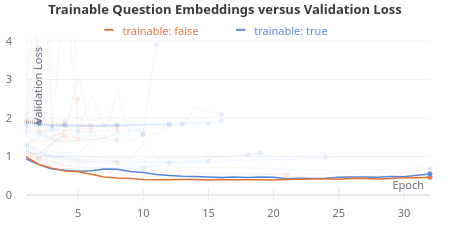
\includegraphics[width=\textwidth]{hyperparam_trainable_question_embedding_loss.png}
        \label{fig:hyperparam_trainable_question_embedding_loss}
        \caption{Validation Loss}
    \end{subfigure}
    \begin{subfigure}[r]{0.49\textwidth}
        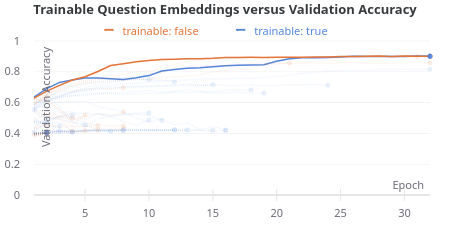
\includegraphics[width=\textwidth]{hyperparam_trainable_question_embedding_accuracy.png}
        \label{fig:hyperparam_trainable_question_embedding_accuracy}
        \caption{Validation Accuracy}
    \end{subfigure}
    \caption{}
    \label{fig:hyperparam_trainable_question_embedding_loss_and_accuracy}
\end{figure}
 
\begin{figure}
    \centering
    \begin{subfigure}[l]{0.5\textwidth}
        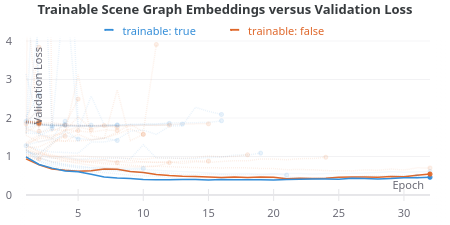
\includegraphics[width=\textwidth]{hyperparam_trainable_scene_embedding_loss.png}
        \label{fig:hyperparam_trainable_scene_embedding_loss}
        \caption{Validation Loss}
    \end{subfigure}
    \begin{subfigure}[r]{0.49\textwidth}
        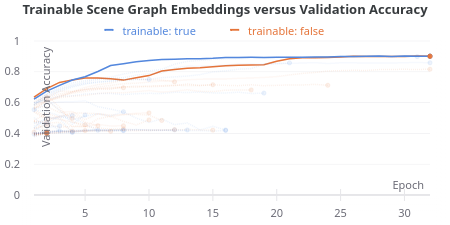
\includegraphics[width=\textwidth]{hyperparam_trainable_scene_embedding_accuracy.png}
        \label{fig:hyperparam_trainable_scene_embedding_accuracy}
        \caption{Validation Accuracy}
    \end{subfigure}
    \caption{}
    \label{fig:hyperparam_trainable_scene_embedding_loss_and_accuracy}
\end{figure}

\begin{figure}
    \centering
    \begin{subfigure}[l]{0.5\textwidth}
        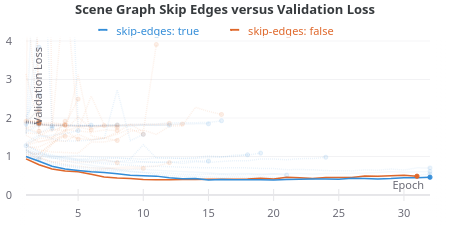
\includegraphics[width=\textwidth]{hyperparam_skip_edges_loss.png}
        \label{fig:hyperparam_skip_edges_loss}
        \caption{Validation Loss}
    \end{subfigure}
    \begin{subfigure}[r]{0.49\textwidth}
        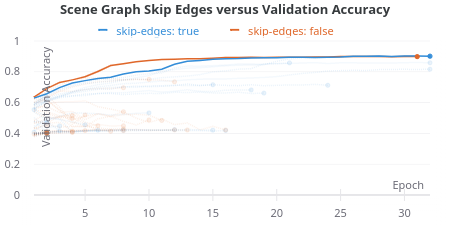
\includegraphics[width=\textwidth]{hyperparam_skip_edges_accuracy.png}
        \label{fig:hyperparam_skip_edges_accuracy}
        \caption{Validation Accuracy}
    \end{subfigure}
    \caption{}
    \label{fig:hyperparam_skip_edges_loss_and_accuracy}
\end{figure}
